\documentclass[aspectratio=169,10pt]{beamer}
\usetheme{default}\usefonttheme{professionalfonts}\setbeamertemplate{navigation symbols}{}\setbeamertemplate{footline}[frame number]
\usepackage[T1]{fontenc}\usepackage[utf8]{inputenc}\usepackage[scaled=0.95]{helvet}\renewcommand{\familydefault}{\sfdefault}\usepackage{booktabs,amsmath}
\setbeamercolor{frametitle}{fg=black}\setbeamercolor{title}{fg=black}
\title{Cars queued behind a cyclist in a shared winter lane}\subtitle{Rue de Terrebonne, winter morning peak}\author{Terrebonne-open-sources (a resident of Côte-des-Neiges--Notre-Dame-de-Grâce)}\date{2026-11-08}
\begin{document}
\frame{\titlepage}
\begin{frame}{The question}\begin{itemize}
\item Winter layout of November 2, 2026: cyclists going with traffic « appelés à partager la voie de circulation avec les véhicules motorisés » (file 1266880005, p.~3).
\item EXP 2023, Figure 6-6: a 3.5\,m lane between two parking lanes.
\item Passing a cyclist needs 1\,m of clearance (art.~341); that lane does not leave it. A driver who catches up stays behind.
\item How many cars build up behind one cyclist at the morning peak?
\end{itemize}\end{frame}
\begin{frame}{The traffic}\centering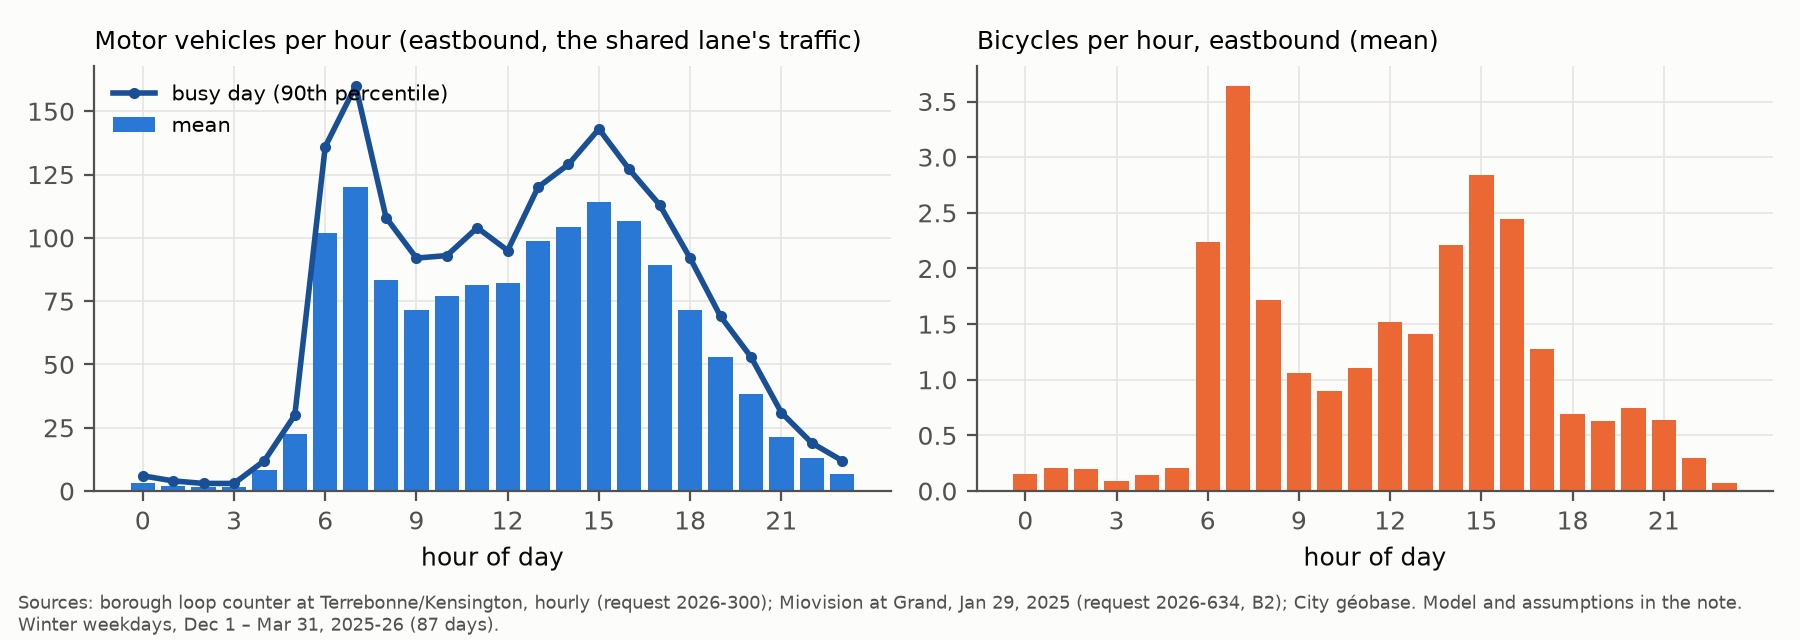
\includegraphics[width=0.95\textwidth]{figures/hourly_flows_en.png}\\\small Kensington loop, 87 winter weekdays: 120 motor vehicles at 07:00--08:00 (busy day 160), 3.6 eastbound bicycles\end{frame}
\begin{frame}{The model}\begin{itemize}
\item Cars catch up at $\lambda = q\,(1/v_b - 1/v_c)$ per km ridden; no passing, so they queue.
\item A queued car leaves when it turns off: share $s$ at each of 17 cross streets in 1.5\,km (Cavendish $\to$ Girouard).
\item Expected queue $N(x) = (\lambda/\mu)(1-e^{-\mu x})$, $\mu = s \times$ cross streets per km; simulation for the spread.
\item Turning off measured at Grand (Jan 29, 2025): 18\,\% at 07:00--09:00; local streets assumed lower (4--12\,\%).
\end{itemize}\end{frame}
\begin{frame}{Three cases}\centering\small
\begin{tabular}{lrrrrrrrr}\toprule
case & $q$ & $v_b$ & $v_c$ & $s$ & caught/km & 0.5\,km & 1\,km & 1.5\,km \\\midrule
low & 100 & 18 & 22 & 12\,\% & 1.0 & 0.4 & 0.6 & 0.7 \\
central & 120 & 15 & 25 & 7\,\% & 3.2 & 1.3 & 2.2 & 2.8 \\
high & 160 & 12 & 28 & 4\,\% & 7.6 & 3.4 & 6.1 & 8.4 \\
\bottomrule\end{tabular}\\[6pt]speeds in km/h, stops included; queue = expected cars behind the cyclist\end{frame}
\begin{frame}{Cars queued behind one cyclist}\centering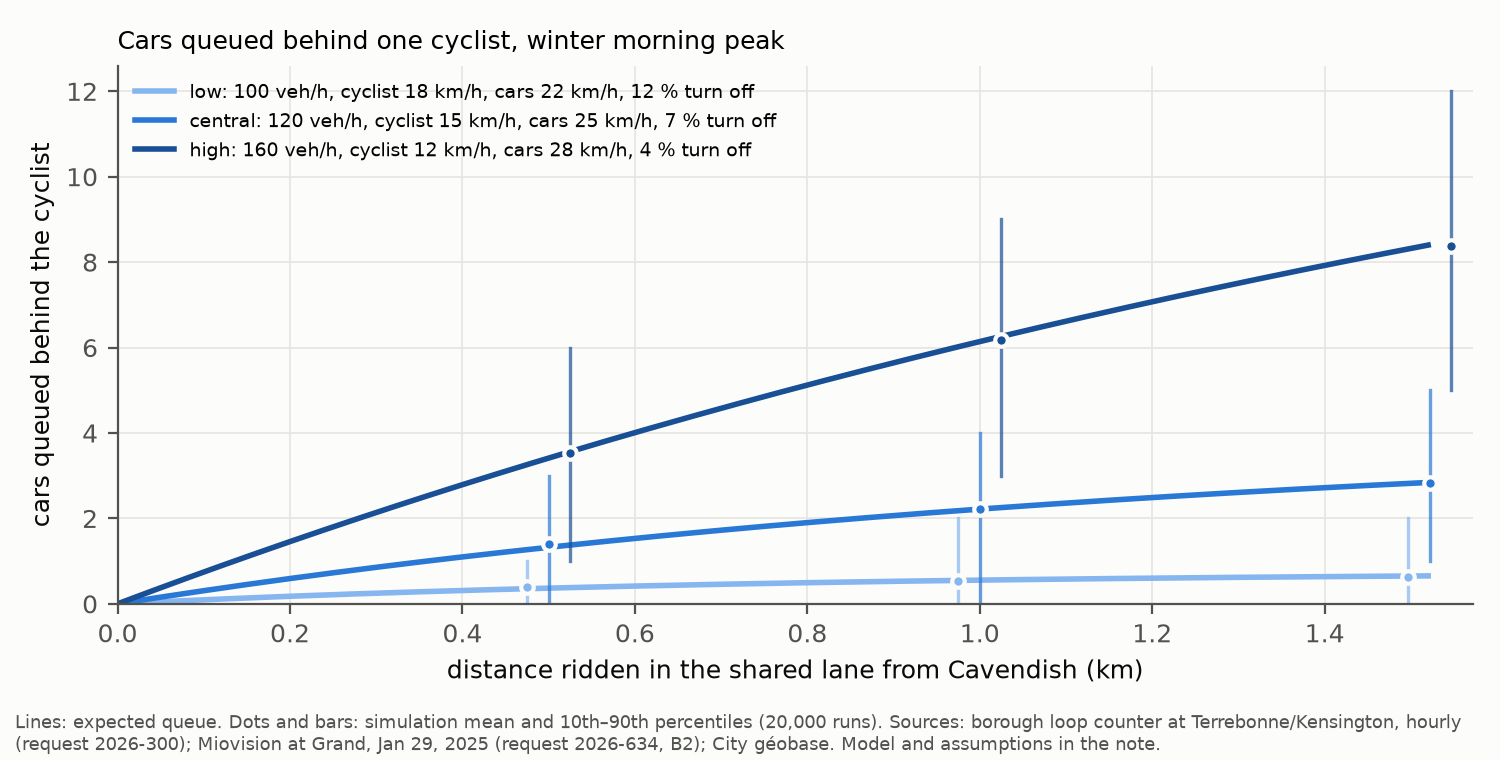
\includegraphics[width=0.9\textwidth]{figures/queue_by_distance_en.png}\end{frame}
\begin{frame}{The result}\begin{itemize}
\item Central case: 2.2 cars after 1\,km, 2.8 at Girouard (simulation median 3, 10th--90th 1--5).
\item Busy morning, slow cyclist: 8.4 at Girouard; quiet morning, fast cyclist: under one.
\item Drivers\textquoteright{} side: about 12 of 120 peak-hour cars (10\,\%) follow a cyclist, each losing at most 1.6\,min/km.
\end{itemize}\end{frame}
\begin{frame}{What drives it}\centering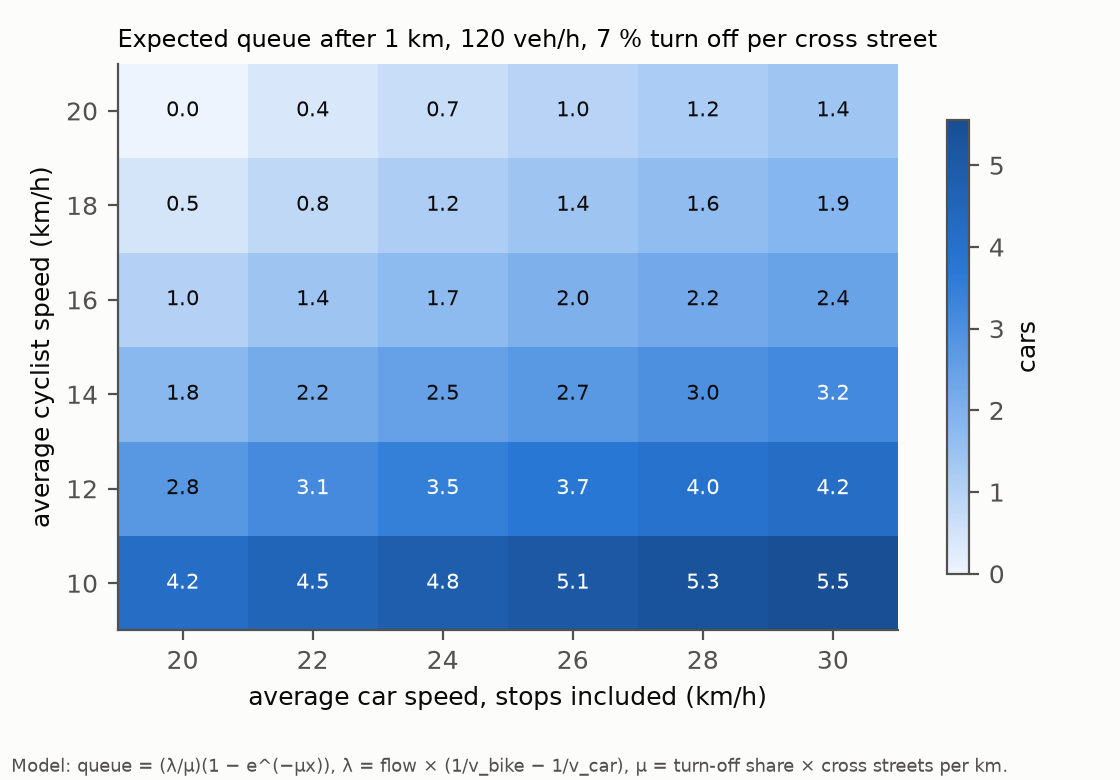
\includegraphics[width=0.62\textwidth]{figures/sensitivity_1km_en.png}\\\small the gap between the two speeds matters most\end{frame}
\begin{frame}{Limits}\begin{itemize}
\item Speeds assumed, not measured; turning off measured at one intersection.
\item No passing assumed; on a vélorue art.~496.3 lets a driver pass where judged safe (shorter queue, closer passes).
\item One cyclist at a time; snowbanks narrow the lane further; west of Cavendish not covered (no comparable count).
\item Code, data and tables: \url{https://github.com/OpenMobilityData/Terrebonne-open-sources/tree/main/2026-shared-lane-queue}
\end{itemize}\end{frame}
\end{document}
